 \documentclass{article} 

\usepackage{amsmath}
\usepackage{amssymb}
\usepackage{latexsym}
\usepackage{fullpage}
\usepackage{enumerate}
\usepackage{graphicx}
\usepackage{mathrsfs}


% The only difference between \newcommand and \renewcomand is that the former is for
% a brand new command, while the later is for a command that is already defined by the
% system, which you plan to use for something else.
\renewcommand{\l}{\left(}
\renewcommand{\r}{\right)}
\renewcommand{\a}{\alpha}
\renewcommand{\b}{\beta}
\newcommand{\g}{\gamma}
\newcommand{\G}{\Gamma}
\renewcommand{\d}{\delta}
\newcommand{\D}{\Delta}
\newcommand{\e}{\epsilon}
\newcommand{\La}{\Lambda}
\newcommand{\la}{\lambda}
\renewcommand{\O}{\Omega}
\renewcommand{\o}{\omega}
\renewcommand{\th}{\theta}
\newcommand{\Th}{\Theta}
\newcommand{\q}{\quad}
\newcommand{\s}{\sigma}
\newcommand{\pa}{\partial}
\newcommand{\bs}{\boldsymbol}
%\renewcommand{\labelenumi}{\underline{\textbf{Step \arabic{enumi}:}}}


\usepackage[inline]{enumitem}
%\renewcommand{\tabcolsep}{2em}
\renewcommand{\arraystretch}{1.5}

\begin{document}
\noindent
{\large Kirchhoff Loop Example}
\smallskip
\hrule
\kern1pt
\hrule

\bigskip
\bigskip
\bigskip
\noindent
\begin{minipage}{0.6\textwidth}

To the right is a circuit with two batteries and some loops. 
You will use Kirchhoff's rules to analyze the circuit, but first answer the
following fill-in-the-blank questions. \emph{1 point each.}

\begin{enumerate}
	\item Kirchhoff's junction rule is a mathematical expression of\\[2ex] conservation
of \underline{\bf charge}. \\[-1ex]
	\item Kirchhoff's loop rule is a mathematical expression of\\[2ex] conservation
of \underline{\bf energy}.

\end{enumerate}

\end{minipage}
\hspace{6ex}
\begin{minipage}{0.3\textwidth}
\vspace{-1cm}
\begin{center}
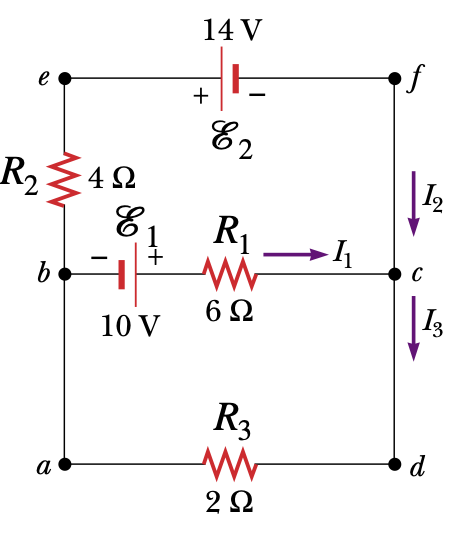
\includegraphics[width=0.95\textwidth]{circuit1}
\end{center}
\end{minipage}\\


\begin{enumerate}

\setcounter{enumi}{2}

\item Also write down an expression relating the currents  $I_1$, $I_2$ and $I_3$
using the ``junction rule''. What junction (e.g., junction $b$) are you considering when you write this? 
\emph{1 point.}\\

\emph{At junction $c$ we write $I_1 + I_2 = I_3$. At junction $b$ we would write the (mathematically
equivalent) $I_3 = I_1 + I_2$.}
\\[.5cm]

\item Using the terms $R_1$, $R_2$, $R_3$, $I_1$, $I_2$, $I_3$, $\mathscr{E}_1$ 
and $\mathscr{E}_2$ write down ``loop rule'' expressions for at least two different
loops. State explicitly what the loop is by giving the order of its corners (e.g. $abcda$). 
\emph{5 points}.\\

\emph{For the loop `$aefda$' we have
\[
- I_2 R_2 - \mathscr{E}_2 - I_3 R_3 = 0.
\]
For the loop `$abcda$' we have
\[
 \mathscr{E}_1 - I_1 R_1 - I_3 R_3 = 0.
\]
For the loop `$befcb$' we have
\[
- I_2 R_2 - \mathscr{E}_2 + I_1 R_1  - \mathscr{E}_1  = 0.
\]
Note that subtracting loop `$abcda$' from loop `$aefda$' gives loop `$befcb$'. So, the three loops are not
linearly independent.}

\newpage 
\item What are the numerical values of the three currents $I_1$, $I_2$, and $I_3$?
\textbf{Show your work}. (\emph{Note:} You may use Wolfram Alpha or another online calculator 
to check your math. But for full credit, show how you eliminate variables to get down to
equations with only one unknown.)
\emph{8 points.}\\[1cm]

\noindent
\emph{We have three equations for three unknowns ($I_1$, $I_2$, and $I_3$),
\[
I_3 = I_1 + I_2, \qquad
- I_2 R_2 - \mathscr{E}_2 - I_3 R_3 =0, \quad {\rm and} \quad
 \mathscr{E}_1 - I_1 R_1 - I_3 R_3 = 0.
\]
Let's use the junction condition to remove $I_3$ from the two loop equations
\[
- I_2 R_2 - \mathscr{E}_2 - (I_1 + I_2) R_3 =0, \qquad
 \mathscr{E}_1 - I_1 R_1 - (I_1 + I_2) R_3 = 0,
\]
or
\[
- I_2 (R_2 + R_3) - \mathscr{E}_2 - I_1 R_3 =0, \qquad
 \mathscr{E}_1 - I_1 (R_1 + R_3) -  I_2 R_3 = 0.
\]
In this case we will benefit from plugging in for the resistances and emfs, so
\[
- I_2 \cdot 6 \ \Omega - 14 \ {\rm V} - I_1 \cdot 2 \ \Omega =0, \qquad
10 \ {\rm V} - I_1 \cdot 8 \ \Omega -  I_2 \cdot 2 \ \Omega = 0.
\]
Multiply the second equation by $-$3 and get
\[
-30 \ {\rm V} +I_1 \cdot 24 \ \Omega +  I_2 \cdot 6 \ \Omega = 0.
\]
Add it to the first equation to get
\[
-44 \ {\rm V} + I_1 \cdot 22 \ \Omega =0, \qquad \Longrightarrow \qquad I_1 = 2 \ {\rm A}.
\]
Plug this into second equation so,
\[
10 \ {\rm V} - 2 \ {\rm A} \cdot 8 \ \Omega -  I_2 \cdot 2 \ \Omega = 0
\qquad \Longrightarrow \qquad -6 \ {\rm V} -  I_2 \cdot 2 \ \Omega = 0
\qquad \Longrightarrow \qquad I_2 = -3 \ {\rm A}.
\]
Finally, from the junction condition we have
\[
I_3 = 2 \ {\rm A} -3 \ {\rm A} = -1 \ {\rm A}.
\]
}

\end{enumerate}

\end{document}

